\documentclass[a4paper,12pt]{article}
\begin{document}

Exemplo de documento do latex. 
Aí você poderia compilar no seu overleaf, fazer suas alterações lá e colar o código nesse arquivo aqui, e então dar commit. 
Se estiver tudo certo, a gente aprova e sua branch vira main e assim a gente vai construindo o repositório do artigo :)

As imagens deverão ficar no mesmo arquivo que o arquivo .tex. Tem de ter a mesma estrutura.

\begin{figure}
    \centering
    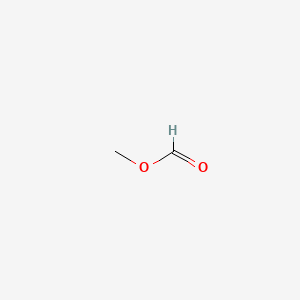
\includegraphics[width=1\linewidth]{imagens/molécula.png}
    \caption{Sei lá molécula aleatória que achei no meu pc.}
    \label{fig:mol}
\end{figure}


\end{document}
